\chapter{MIMO Communication Performance Evaluation}

Having characterized the antenna element and the metasurface transmitarray lens individually in the preceding chapter, this chapter evaluates the system-level communication performance that results when they are deployed together in a multi-antenna link. The evaluation is carried out with Sionna-RT, a differentiable ray-tracing framework that reconstructs the wireless channel between transmitters and receivers from the propagation environment's geometry and material properties, allowing the antenna far-field patterns obtained in Chapter~2 to be embedded directly into a physically realistic multipath channel rather than an idealized analytical one. To capture how this channel behaves under realistic user distributions rather than at a single, arbitrarily chosen link geometry, a Monte Carlo methodology is adopted: transmitter positions are drawn at random within a $20\,\text{m}\times20\,\text{m}\times3\,\text{m}$ indoor room across many independent drops, and the resulting channel realizations are aggregated to obtain statistically representative capacity, delay-spread, and channel-conditioning metrics. This setup is used first to isolate the effect of the antenna lens by comparing it against a conventional coplanar array under identical transmitter geometries, and then to examine how the resulting performance scales as the receive array is extended to higher-order MIMO configurations.

\section{Comparison of Different Antenna Placements}\label{sec:comparison-antenna-placements}

This section quantifies the antenna lens's effect on the multi-user MIMO channel by comparing two RX configurations under an identical TX geometry: a conventional coplanar array without the lens, and the antenna lens-assisted focal-plane configuration. A paired Monte Carlo methodology evaluates the same twenty drops of nine randomly placed transmitters under both RX configurations and nine RX angles ($+60^\circ$ to $-60^\circ$ in $15^\circ$ steps), yielding 180 result rows per configuration, so that any difference in outcome is attributable to the RX pattern alone rather than to differing TX placement. The simulation parameters are summarized below; all reported results were cross-validated using two independent implementations of the analysis procedure.

Interpreting this comparison correctly requires clarifying what the nine RX labels physically represent, since the two configurations realize them very differently (Figure~\ref{fig:mc9x9-rx-placement}). With the lens (Fig.~\ref{fig:mc9x9-rx-placement}(a)), the nine labels are nine steering states of a single physical receiver, so the corresponding RX points cluster within a few centimeters of each other. Without the lens (Fig.~\ref{fig:mc9x9-rx-placement}(b)), the same count instead corresponds to nine physically separate coplanar patch elements sharing one fixed $0^\circ$ far-field pattern -- the conventional baseline against which the steerable lens is compared.

\begin{figure}[htbp]
    \centering
    \begin{minipage}{0.75\textwidth}
        \centering
        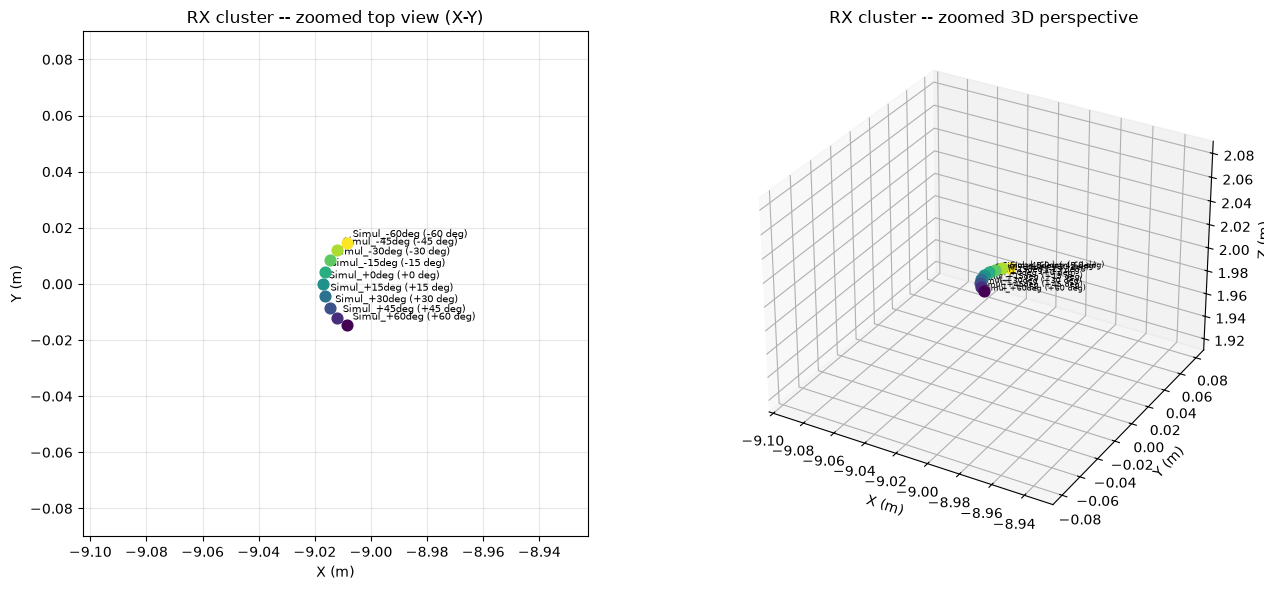
\includegraphics[width=\linewidth]{Images/3_1_PositionofReceiverAntennaLens.png}
        (a)
    \end{minipage}

    \vspace{0.5em}
    \begin{minipage}{0.75\textwidth}
        \centering
        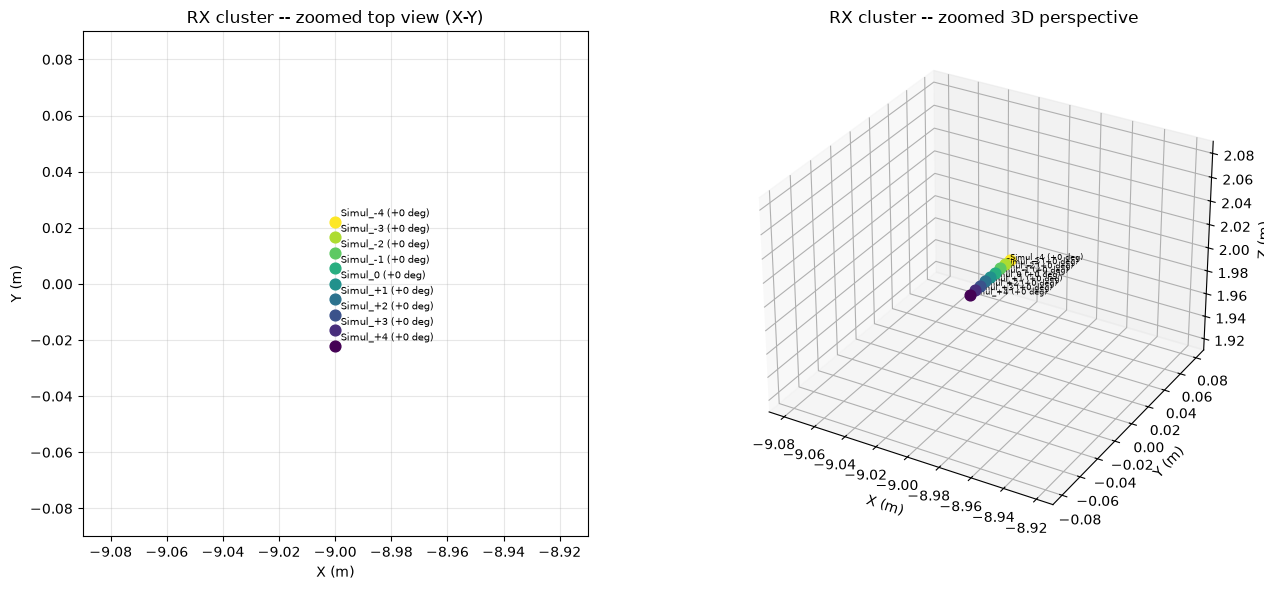
\includegraphics[width=\linewidth]{Images/3_1_PositionofReceiverWOAntennaLens.png}
        (b)
    \end{minipage}
    \caption{Physical RX placement (top view and zoomed 3D perspective): (a) lens-assisted receiver, nine lens-steering scenarios clustered at a single physical location; (b) conventional receiver, nine physically distinct coplanar patch elements sharing a common $0^\circ$ pattern.}
    \label{fig:mc9x9-rx-placement}
\end{figure}

This same sensitivity to geometry motivates the Monte Carlo approach itself: because capacity, delay spread, and conditioning all depend on the relative TX-RX position, a single fixed transmitter location could over- or under-state the lens's benefit purely by chance. Drawing 180 TX positions (20 drops $\times$ 9 TX) across the $20\,\text{m}\times20\,\text{m}$ floor plan (Figure~\ref{fig:mc9x9-tx-montecarlo}) instead yields a realistic distribution of user locations relative to the fixed RX cluster, so the reported metrics reflect expected system performance rather than one favorable or unfavorable placement.

\begin{figure}[htbp]
    \centering
    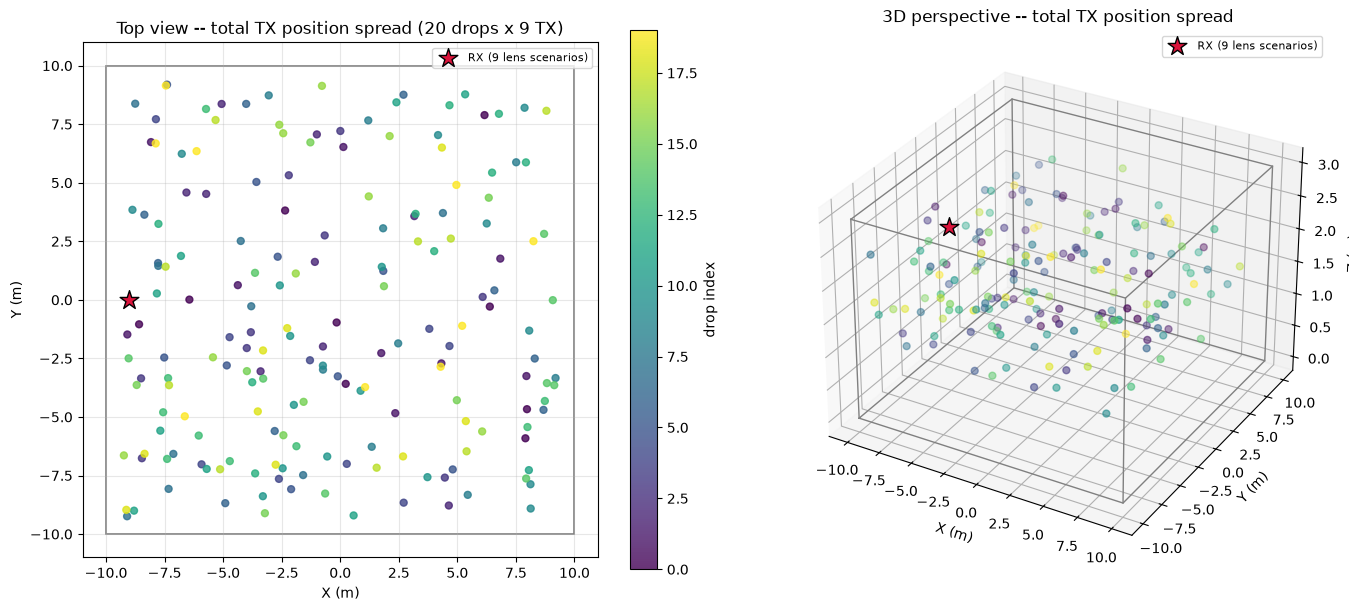
\includegraphics[width=0.9\linewidth]{Images/3_1_PositionofTXMonteCarloPosition.png}
    \caption{Monte Carlo TX position sampling: top view and 3D perspective of the 180 randomized transmitter positions (20 drops $\times$ 9 TX) spread across the $20\,\text{m}\times20\,\text{m}$ room, relative to the fixed RX cluster (star).}
    \label{fig:mc9x9-tx-montecarlo}
\end{figure}

\begin{itemize}
    \item \textbf{RX pattern}: patch far-field, identical for every angle (without lens) vs.\ HFSS far-field pattern per lens angle (with lens)
    \item \textbf{TX pattern}: isotropic, with the same 9 random positions per drop reused across both configurations
    \item \textbf{Room size}: $20\,\text{m}\times20\,\text{m}\times3\,\text{m}$
    \item \textbf{Carrier / bandwidth}: 38~GHz, 400~MHz (401 frequency points)
    \item \textbf{Path samples per source}: 100{,}000 (recommended final value: 1{,}000{,}000)
\end{itemize}

\subsection{Evaluation Metrics}

Four groups of metrics characterize the channel. First, since the nine transmitters act as independent (non-coherent) sources, the received power at frequency bin $f$ is the sum of their individual contributions,
\begin{equation}
    P_\mathrm{RX}(f) = P_\mathrm{TX}\sum_{i=1}^{9}\left|H_i(f)\right|^2,
    \label{eq:mc9x9-prx}
\end{equation}
where $H_i(f)$ is the channel response from transmitter $i$ and $P_\mathrm{TX}$ is the per-transmitter power. With thermal noise power $P_\mathrm{N}=kTB\cdot10^{\mathrm{NF}/10}$, the resulting SNR and equivalent SISO channel capacity, averaged over $N_f$ frequency points, follow the Shannon bound,
\begin{equation}
    \mathrm{SNR}(f) = \frac{P_\mathrm{RX}(f)}{P_\mathrm{N}}, \qquad
    C = \frac{1}{N_f}\sum_{f}\log_2\!\left(1+\mathrm{SNR}(f)\right),
    \label{eq:mc9x9-capacity}
\end{equation}
with the corresponding ideal throughput given by $\mathrm{Throughput}=B\times C$, where $B$ is the system bandwidth. Second, the wideband delay dispersion is obtained from the power-delay profile formed by summing the inverse-Fourier-transformed responses of the nine transmitters,
\begin{equation}
    \mathrm{PDP}(\tau)=\sum_{i=1}^{9}\left|\mathrm{IFFT}_f\{H_i(f)\}\right|^2,
    \label{eq:mc9x9-pdp}
\end{equation}
from which the RMS delay spread $\tau_\mathrm{rms}$ is computed as the second central moment of $\mathrm{PDP}(\tau)$ about its mean delay. Third, to assess channel conditioning and spatial-multiplexing potential, the nine RX-angle channels of a given drop are stacked into a virtual $9\times9$ matrix $\mathbf{H}(f)$ and decomposed by SVD, $\mathbf{H}(f)=\mathbf{U}\boldsymbol\Sigma\mathbf{V}^{H}$, with singular values $\sigma_1(f)\ge\dots\ge\sigma_9(f)$. The condition number and effective rank follow as
\begin{equation}
    \kappa(f) = \frac{\sigma_1(f)}{\sigma_9(f)}, \qquad
    \mathrm{erank}(f) = \exp\!\left(-\sum_{i} p_i(f)\ln p_i(f)\right), \qquad
    p_i(f) = \frac{\sigma_i(f)^2}{\sum_{j}\sigma_j(f)^2},
    \label{eq:mc9x9-condrank}
\end{equation}
where $\mathrm{erank}(f)$ is the Shannon entropy of the normalized eigenmode energy distribution; a well-conditioned, fully multiplexing-capable channel has $\kappa(f)\to1$ and $\mathrm{erank}(f)\to9$. Finally, the virtual $9\times9$ MIMO ergodic capacity at a fixed SNR, with equal power allocated per stream, is
\begin{equation}
    C_\mathrm{MIMO}(\mathrm{SNR}) = \mathbb{E}_f\!\left[\sum_{i=1}^{9}\log_2\!\left(1+\frac{\mathrm{SNR}}{N_t}\,\sigma_i(f)^2\right)\right], \qquad N_t=9,
    \label{eq:mc9x9-mimocapacity}
\end{equation}
reported at $\mathrm{SNR}=10\,\text{dB}$. The nine RX-angle channels used in Equations~\ref{eq:mc9x9-condrank}--\ref{eq:mc9x9-mimocapacity} are not measured simultaneously by a single physical receiver; they are combined into a virtual matrix solely to assess channel diversity and conditioning, not to represent a physically realizable single-receiver MIMO capacity.

\subsection{Standalone Characterization of Each Configuration}

Before the two configurations are combined into a joint comparison, each is first characterized independently over its own 180 rows, as shown in Fig.~\ref{fig:mc9x9-standalone-wolens} (without lens) and Fig.~\ref{fig:mc9x9-standalone-lens} (with lens).

\begin{figure}[htbp]
    \centering
    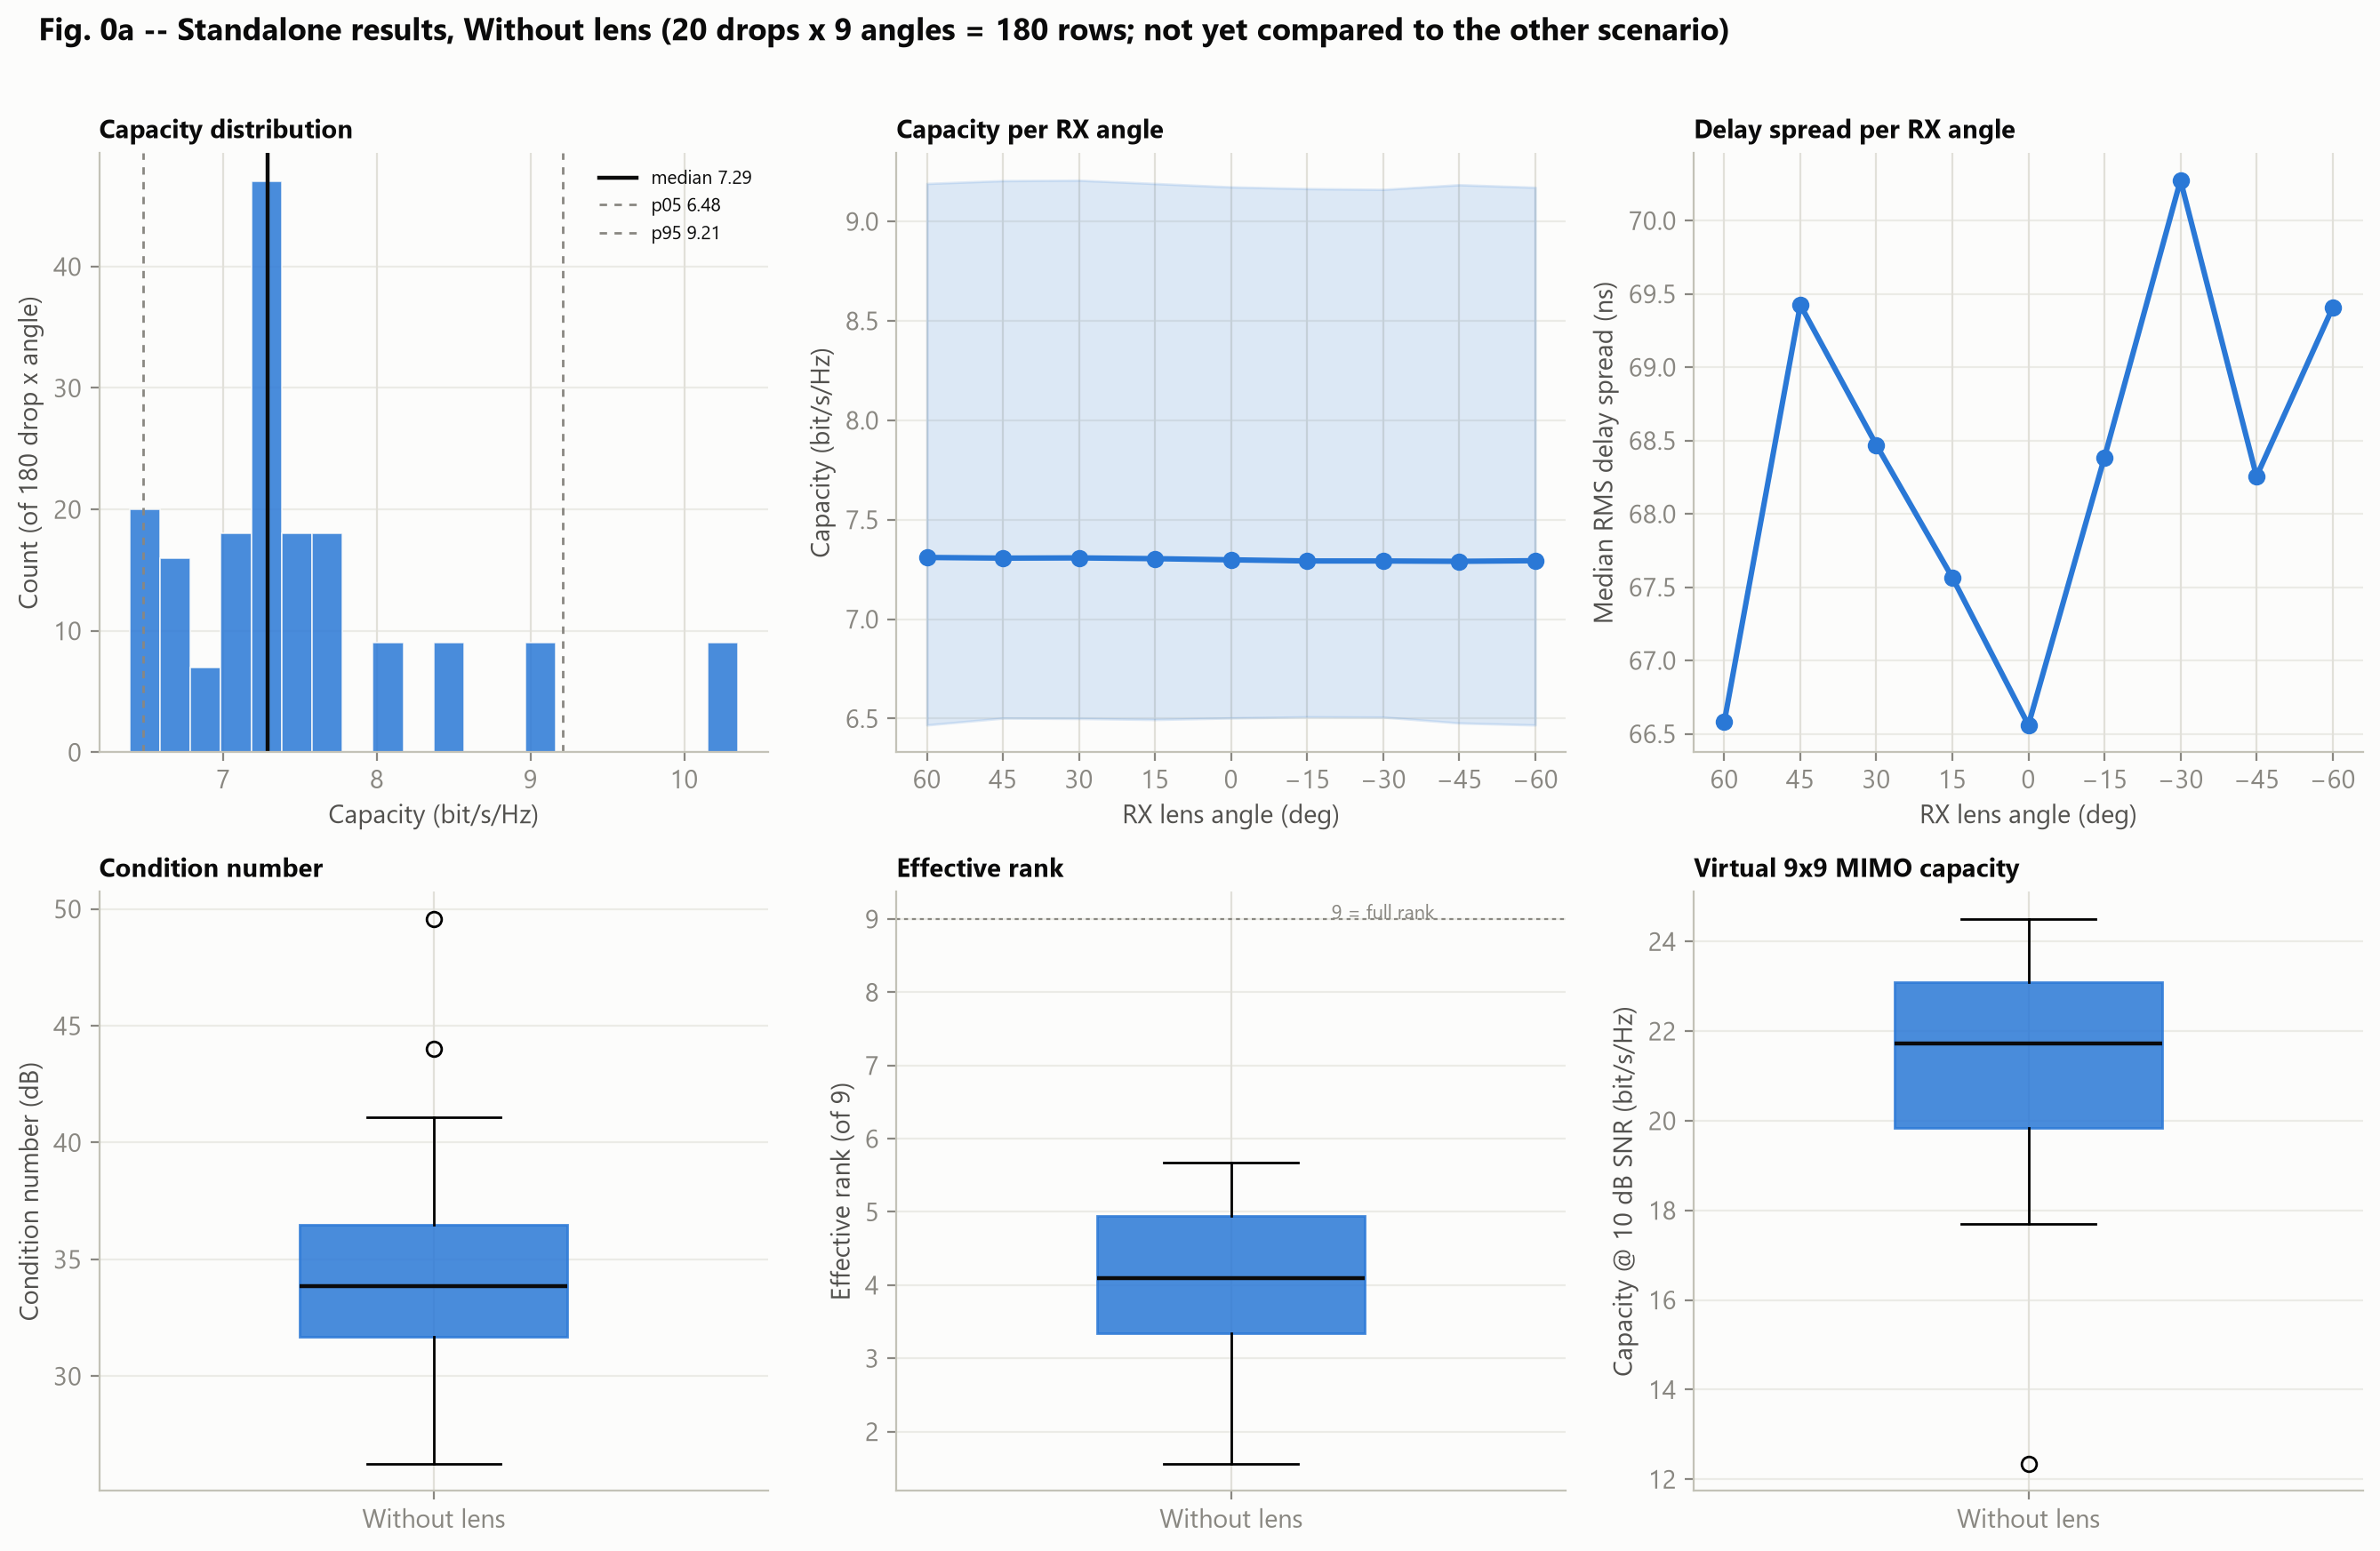
\includegraphics[width=0.85\textwidth]{Images/Eval_20x20_MonteCarlo9x9/asset/figures/fig0a_without_lens_individual.png}
    \caption{Standalone characterization of the conventional coplanar (without-lens) configuration: capacity histogram, capacity per RX angle, RMS delay spread per angle, and virtual $9\times9$ MIMO conditioning.}
    \label{fig:mc9x9-standalone-wolens}
\end{figure}

Without the lens, the channel is close to a flat baseline across all angles, since the RX pattern is identical regardless of angle label: median capacity is 7.29~bit/s/Hz (5th/95th percentile 6.48/9.21), median RMS delay spread is 68.29~ns, and the virtual $9\times9$ MIMO conditioning yields a median condition number of 49.4 (33.8~dB) and a median effective rank of only 4.09 of 9.

\begin{figure}[htbp]
    \centering
    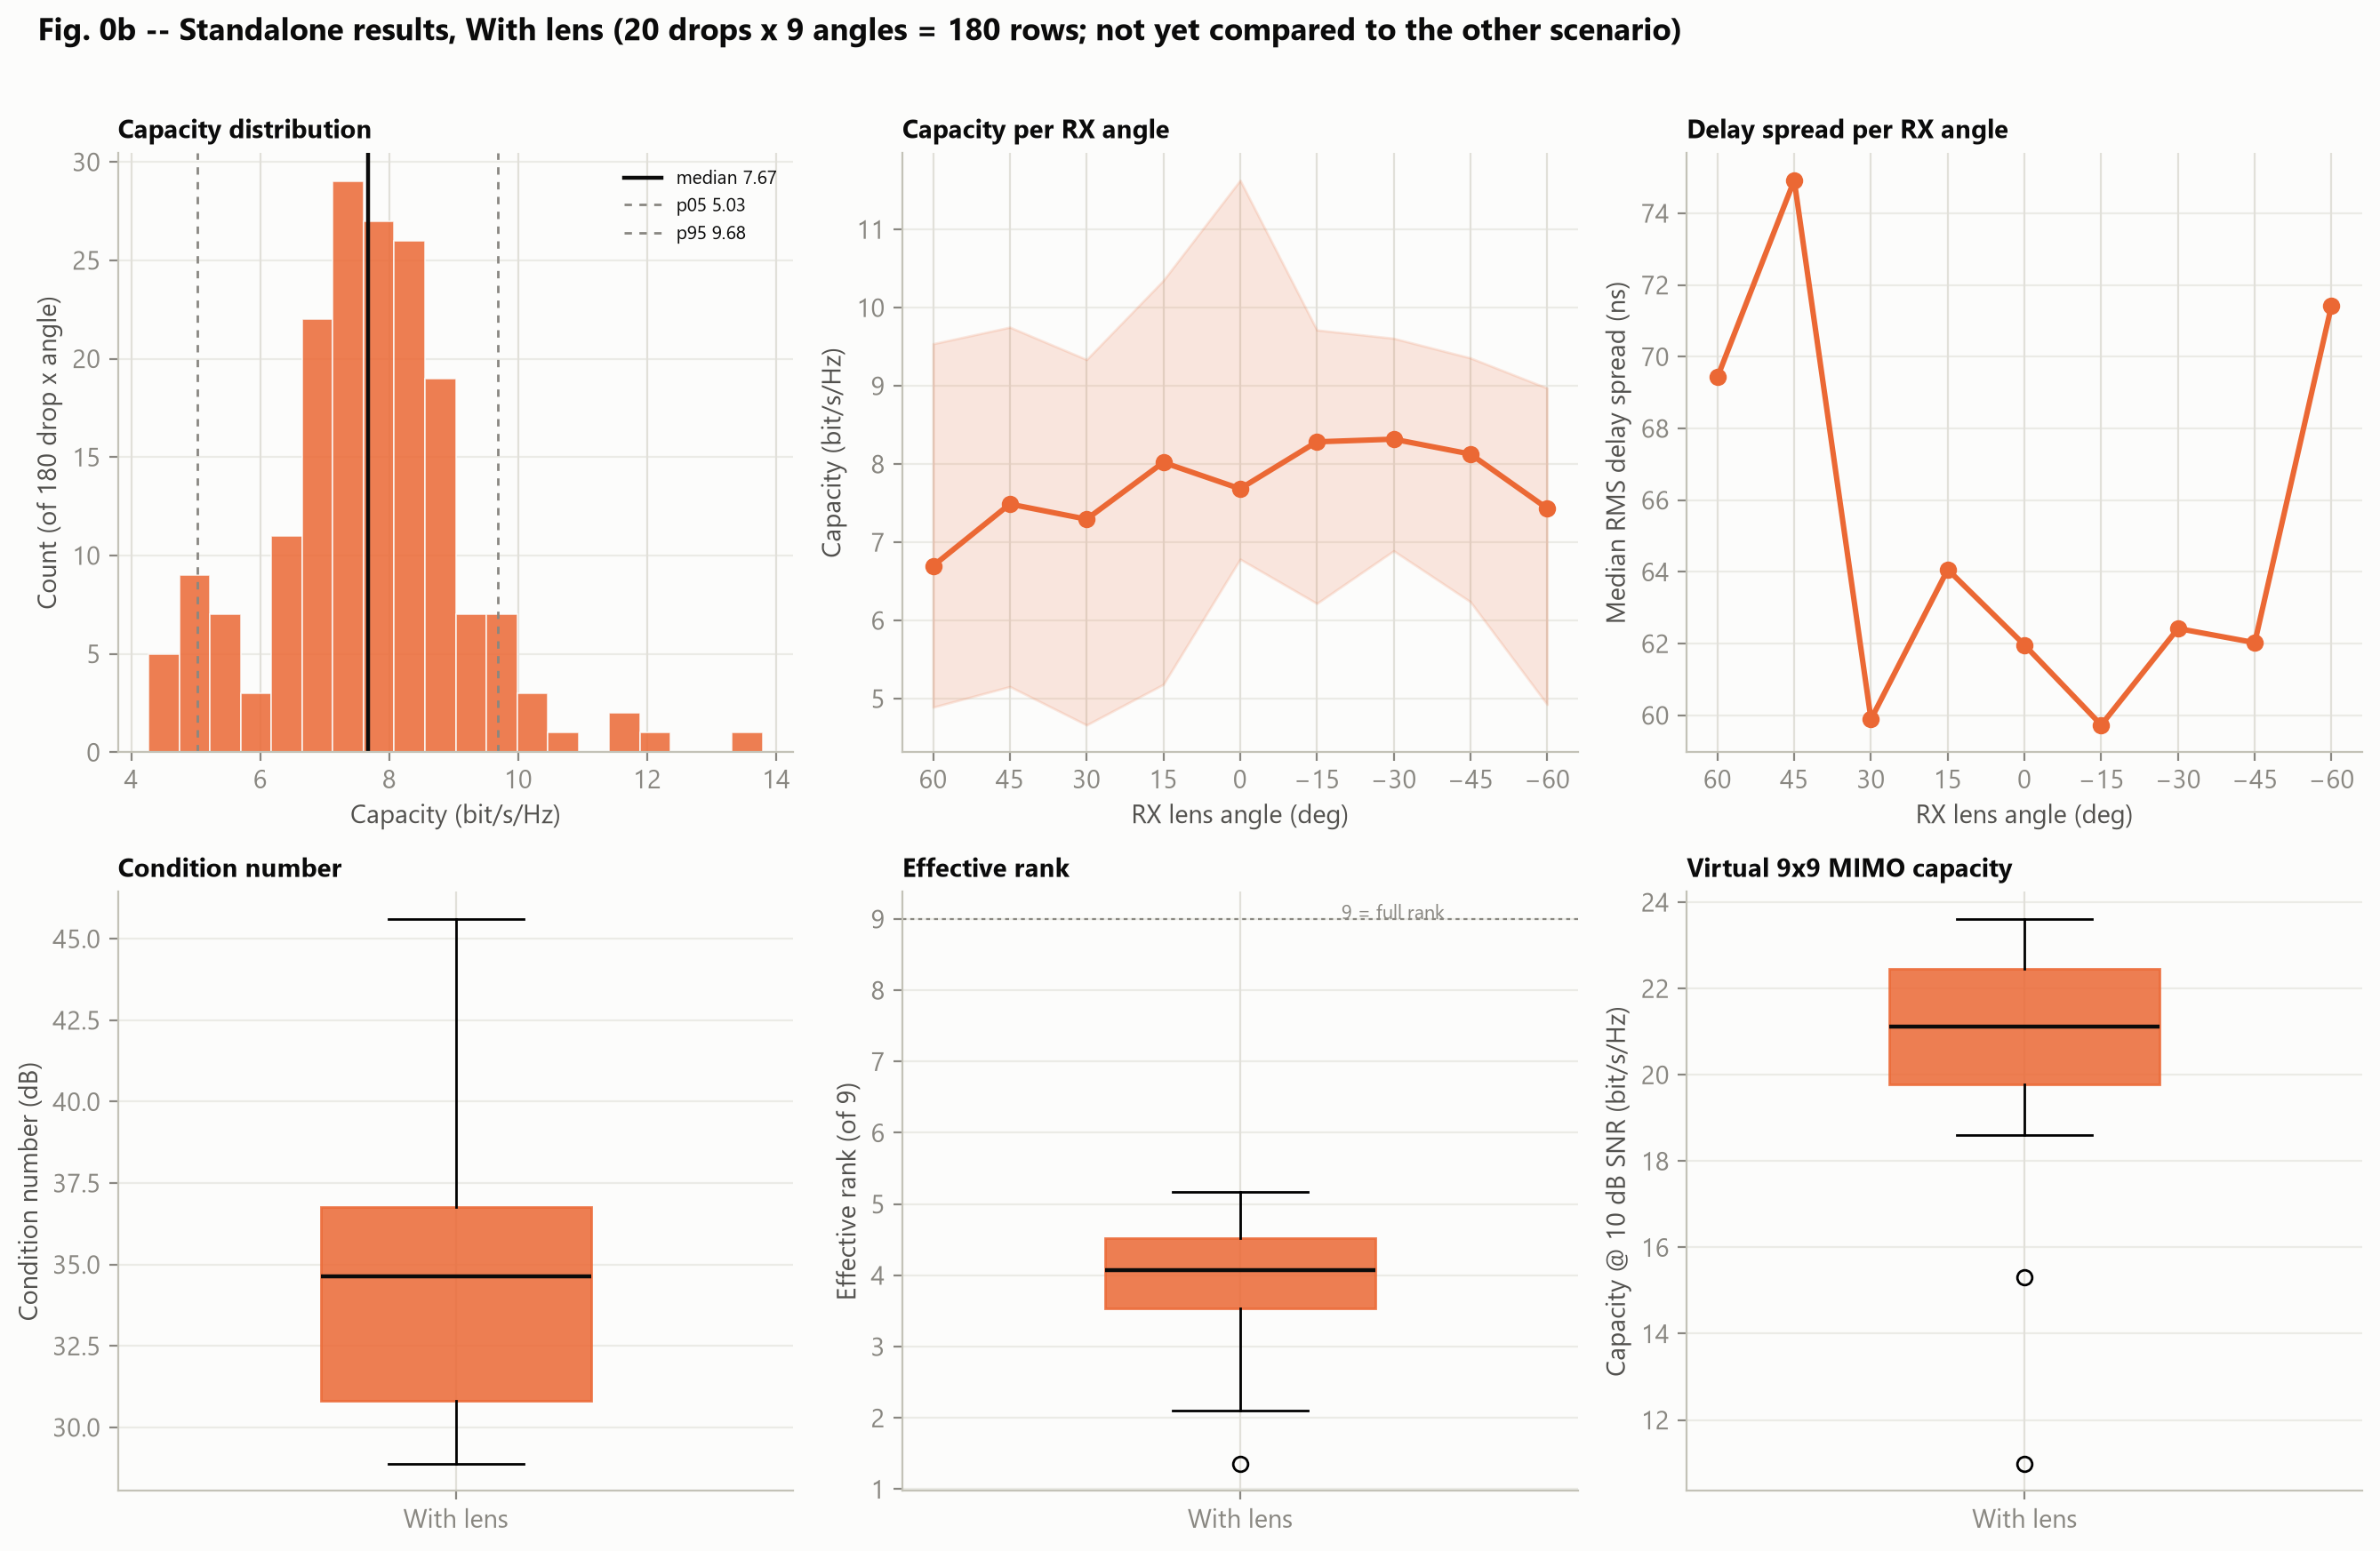
\includegraphics[width=0.85\textwidth]{Images/Eval_20x20_MonteCarlo9x9/asset/figures/fig0b_with_lens_individual.png}
    \caption{Standalone characterization of the antenna lens-assisted focal-plane configuration: capacity histogram, capacity per RX angle, RMS delay spread per angle, and virtual $9\times9$ MIMO conditioning.}
    \label{fig:mc9x9-standalone-lens}
\end{figure}

With the lens, median capacity is higher, at 7.67~bit/s/Hz (5th/95th percentile 5.02/9.68), but the distribution is markedly wider, and capacity is no longer flat across angle: it is lowest near $+60^\circ$ and highest near $-15^\circ$/$-30^\circ$. Median RMS delay spread is lower, at 65.01~ns, while the virtual MIMO conditioning (median effective rank 4.07 of 9) is essentially unchanged from the without-lens case, a point examined further below.

\subsection{Channel Capacity Comparison}

\begin{figure}[htbp]
    \centering
    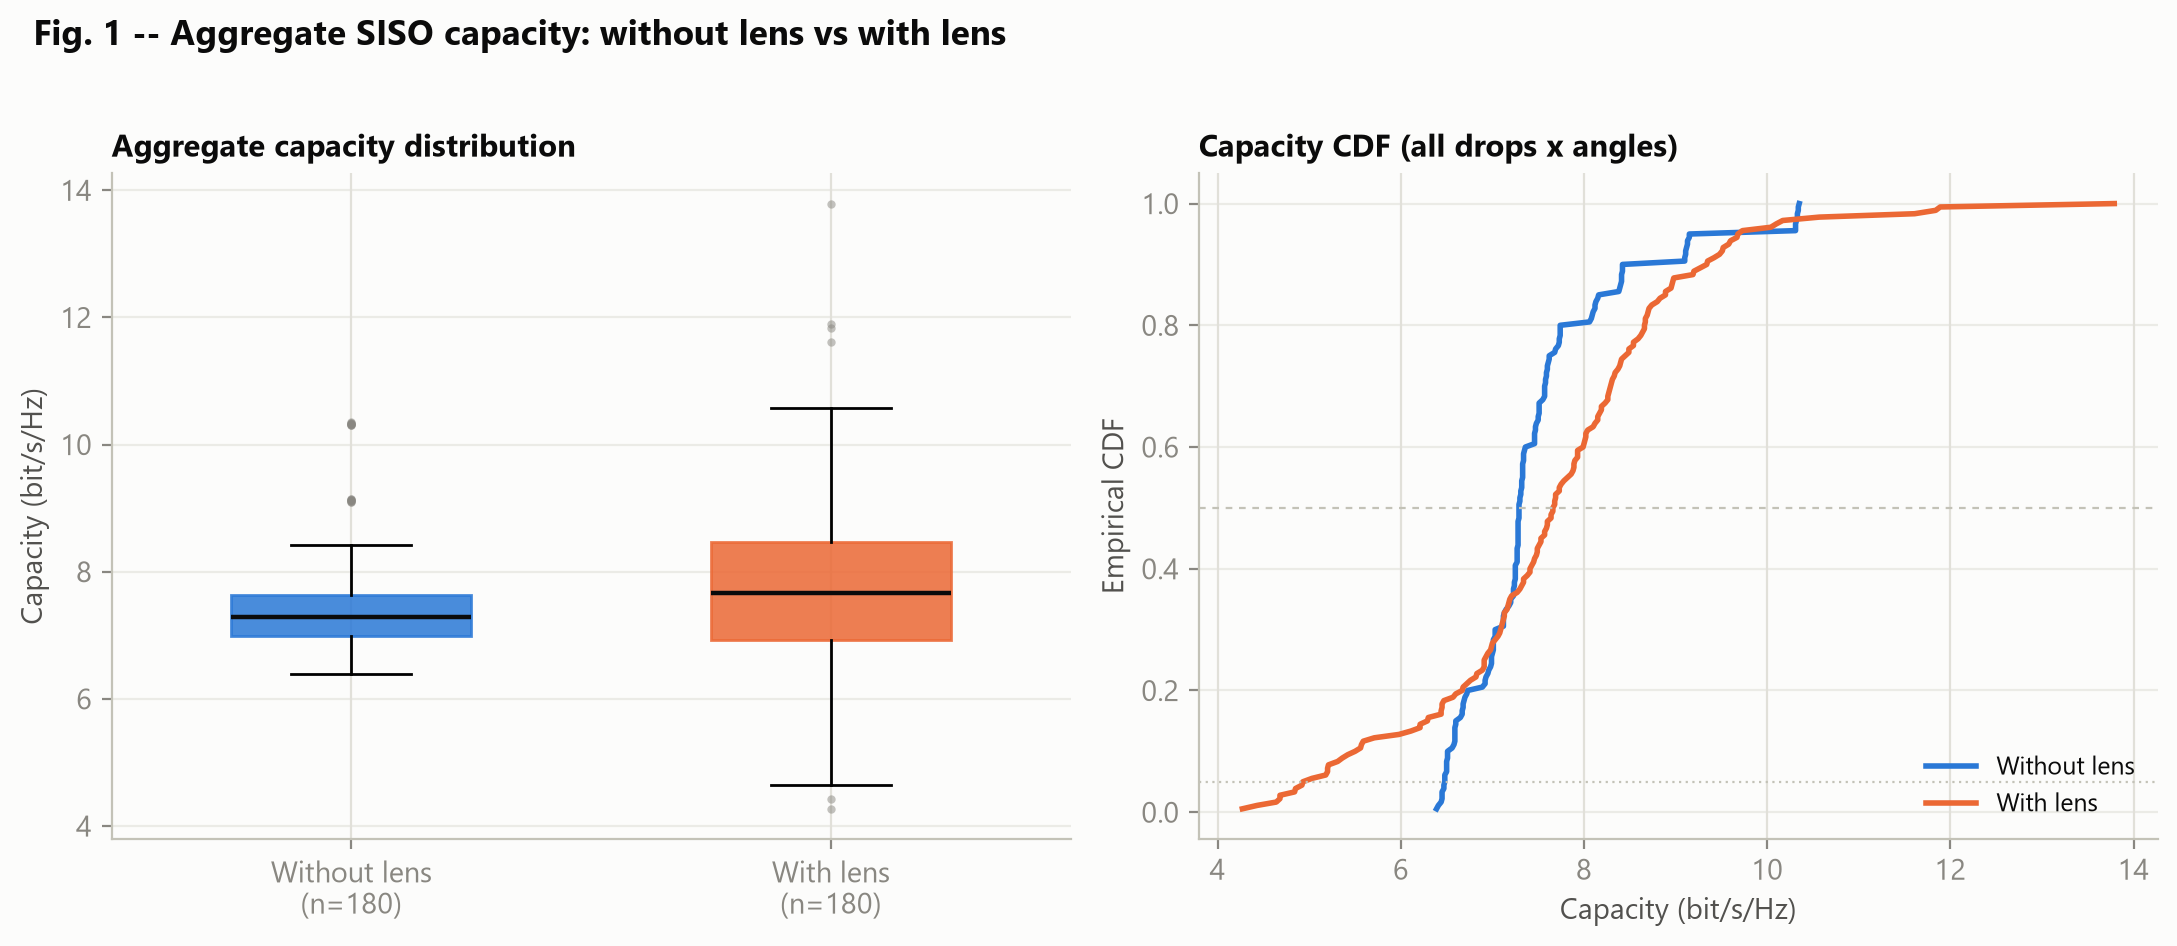
\includegraphics[width=0.85\textwidth]{Images/Eval_20x20_MonteCarlo9x9/asset/figures/fig1_capacity_aggregate.png}
    \caption{Aggregate channel capacity distribution: without lens vs.\ with lens (boxplot and CDF over all 180 rows).}
    \label{fig:mc9x9-capacity-aggregate}
\end{figure}

Table~\ref{tab:mc9x9-aggregate} and Fig.~\ref{fig:mc9x9-capacity-aggregate} compare the aggregate capacity distributions. The lens raises median capacity and ideal throughput by approximately 5\%, but also widens the spread of outcomes: the 5th-percentile capacity drops by 1.46~bit/s/Hz even as the median and 95th percentile improve, consistent with a crossover in the cumulative distribution near 7.3--7.5~bit/s/Hz.

\begin{table}[htbp]
    \centering
    \caption{Aggregate capacity comparison over all 180 rows.}
    \label{tab:mc9x9-aggregate}
    \begin{tabular}{lccc}
        \toprule
        \textbf{Metric} & \textbf{Without lens} & \textbf{With lens} & \textbf{Change} \\
        \midrule
        Median capacity & 7.29~bit/s/Hz & 7.67~bit/s/Hz & $+0.38$ ($+5.2\%$) \\
        5th percentile capacity & 6.48~bit/s/Hz & 5.02~bit/s/Hz & $-1.46$ \\
        95th percentile capacity & 9.21~bit/s/Hz & 9.68~bit/s/Hz & $+0.47$ \\
        Median ideal throughput & 2.92~Gbit/s & 3.07~Gbit/s & $+0.15$ ($+5.1\%$) \\
        \bottomrule
    \end{tabular}
\end{table}

\begin{figure}[htbp]
    \centering
    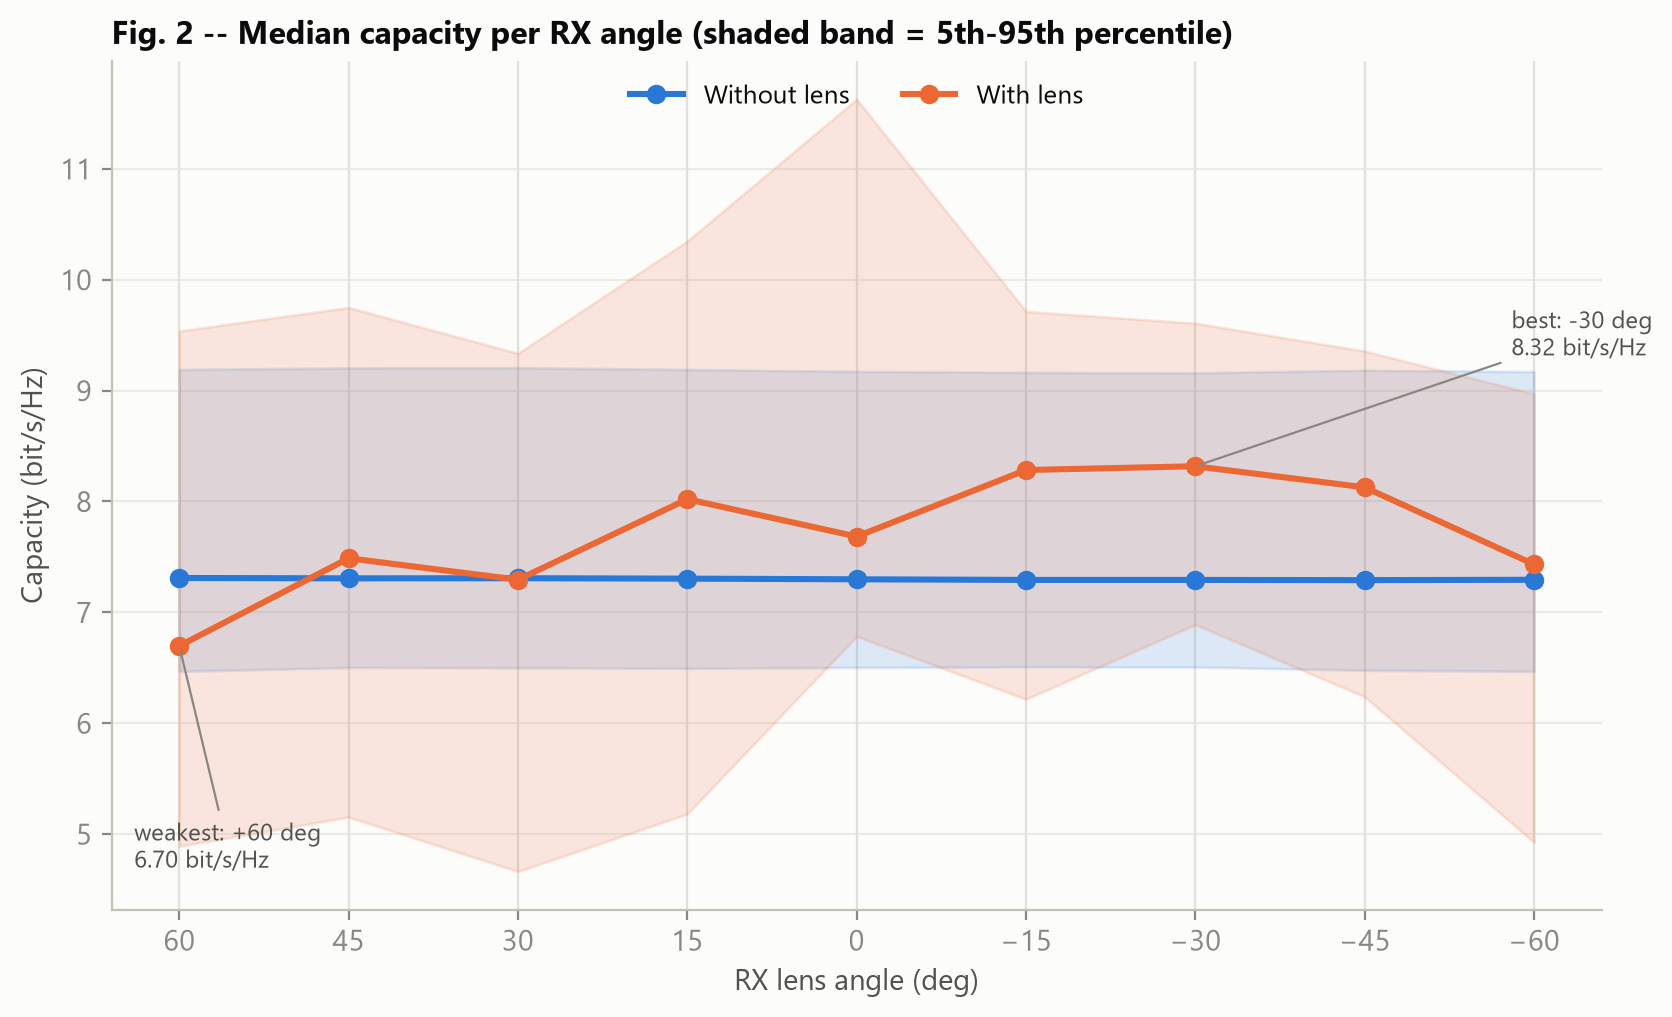
\includegraphics[width=0.85\textwidth]{Images/Eval_20x20_MonteCarlo9x9/asset/figures/fig2_capacity_vs_angle.png}
    \caption{Median channel capacity per RX angle label, without lens vs.\ with lens, with 5th--95th percentile bands.}
    \label{fig:mc9x9-capacity-angle}
\end{figure}

This aggregate improvement, however, masks a strong angular dependence (Table~\ref{tab:mc9x9-per-angle}, Fig.~\ref{fig:mc9x9-capacity-angle}). Without the lens, median capacity remains essentially flat (approximately 7.3~bit/s/Hz) at every angle. With the lens, capacity ranges from 6.70~bit/s/Hz at $+60^\circ$, the weakest angle and worse than without the lens, to 8.32~bit/s/Hz at $-30^\circ$, the best angle -- indicating that the lens acts as a direction-selective gain mechanism rather than a uniform improvement. The response is also asymmetric between positive and negative angles (e.g., $-30^\circ$: 8.32 vs.\ $+30^\circ$: 7.29~bit/s/Hz), suggesting that the underlying angular mapping merits further verification.

\begin{table}[htbp]
    \centering
    \caption{Median channel capacity per RX angle (bit/s/Hz).}
    \label{tab:mc9x9-per-angle}
    \begin{tabular}{lccc}
        \toprule
        \textbf{Angle} & \textbf{Without lens} & \textbf{With lens} & \textbf{Difference} \\
        \midrule
        $+60^\circ$ & 7.31 & 6.70 & $-0.61$ \\
        $+45^\circ$ & 7.31 & 7.49 & $+0.18$ \\
        $+30^\circ$ & 7.31 & 7.29 & $-0.01$ \\
        $+15^\circ$ & 7.30 & 8.02 & $+0.72$ \\
        $0^\circ$   & 7.30 & 7.68 & $+0.39$ \\
        $-15^\circ$ & 7.29 & 8.28 & $+0.99$ \\
        $-30^\circ$ & 7.29 & \textbf{8.32} & \textbf{$+1.03$} \\
        $-45^\circ$ & 7.29 & 8.13 & $+0.84$ \\
        $-60^\circ$ & 7.29 & 7.43 & $+0.14$ \\
        \bottomrule
    \end{tabular}
\end{table}

\begin{figure}[htbp]
    \centering
    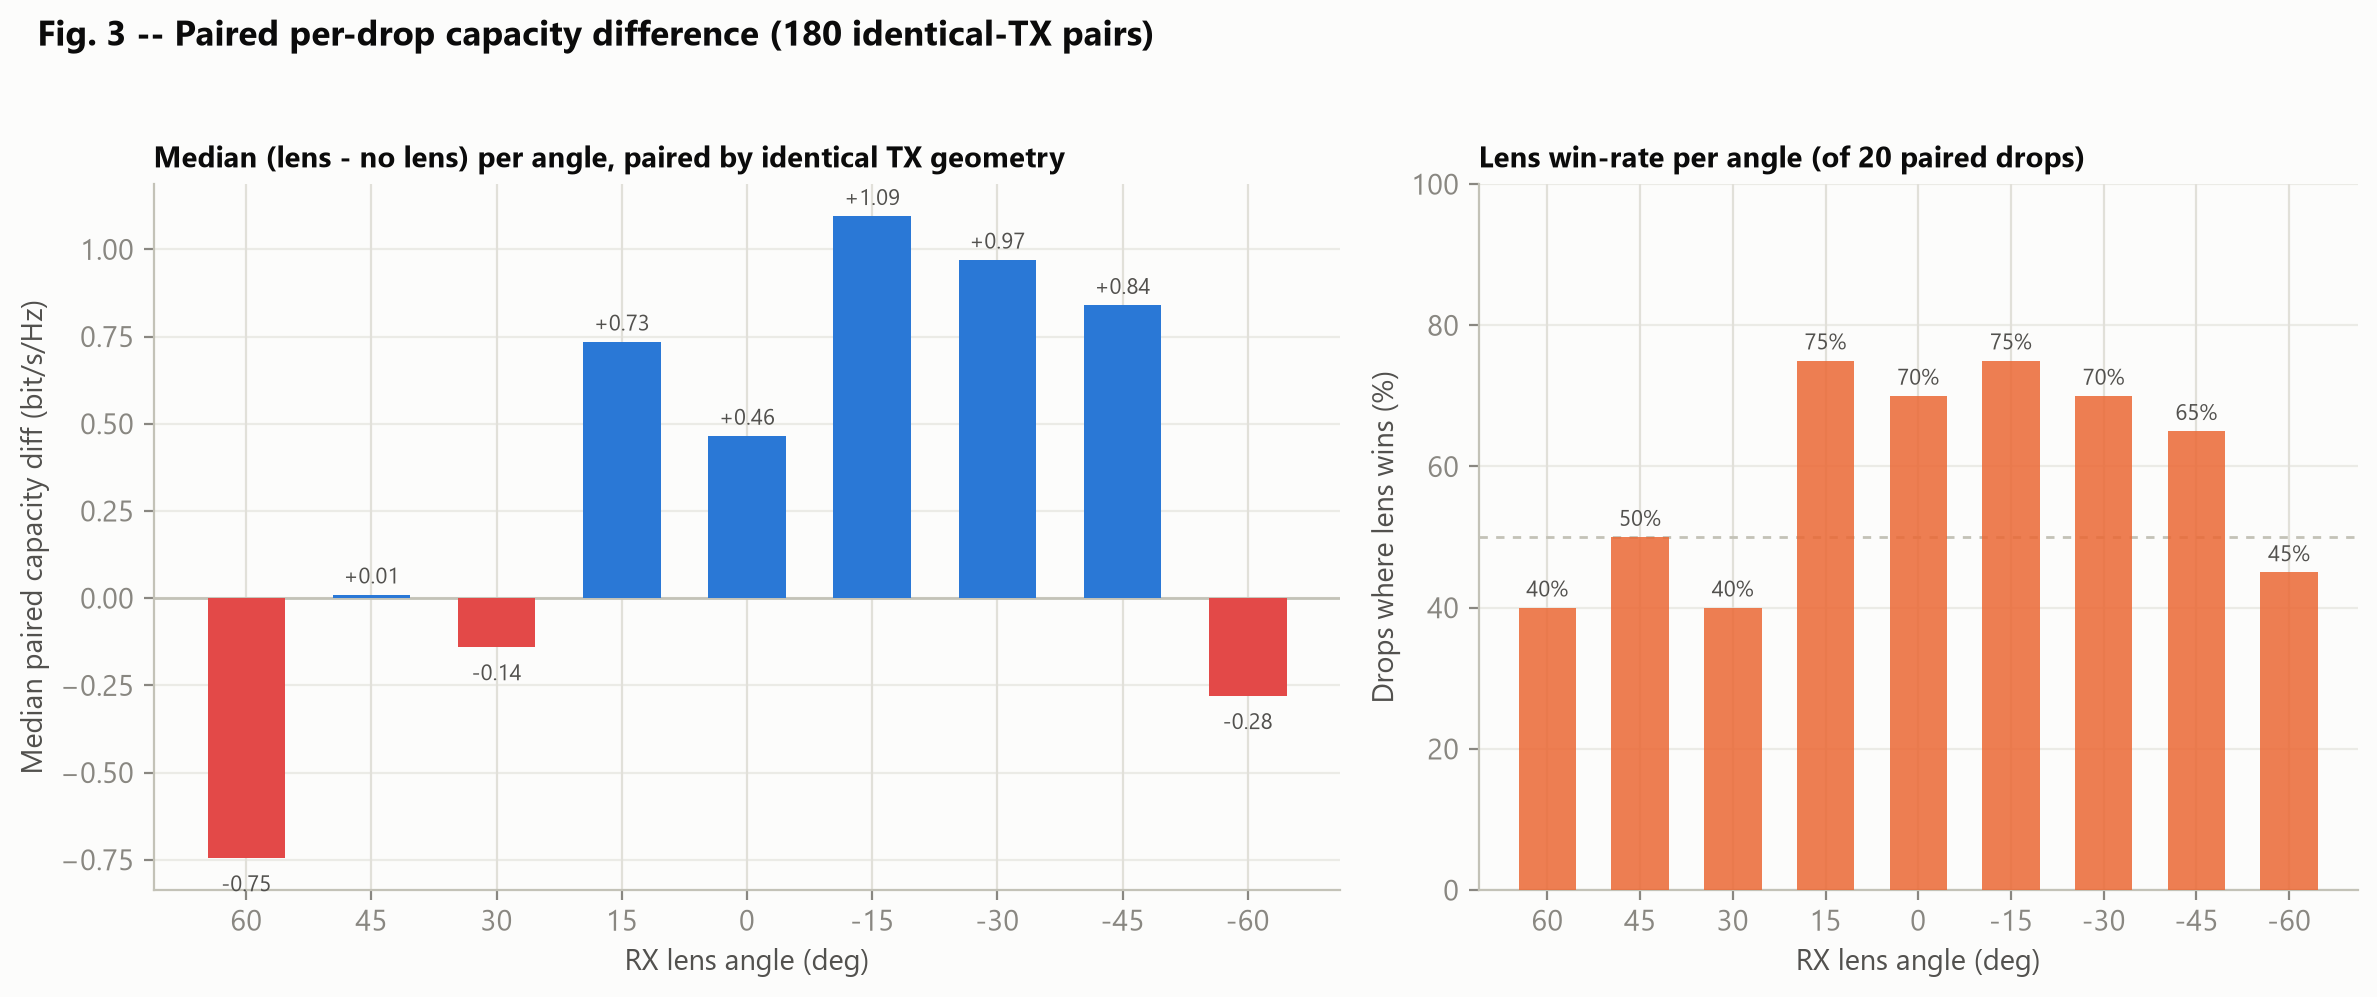
\includegraphics[width=0.85\textwidth]{Images/Eval_20x20_MonteCarlo9x9/asset/figures/fig3_paired_diff_by_angle.png}
    \caption{Paired per-drop capacity difference (with lens minus without lens) by RX angle, and the lens win-rate per angle across the 20 drops.}
    \label{fig:mc9x9-paired-diff}
\end{figure}

Because the transmitter positions are identical across the two configurations, the 180 rows form matched pairs (Fig.~\ref{fig:mc9x9-paired-diff}). The lens yields a median per-pair gain of 0.40~bit/s/Hz and wins in 106 of 180 pairs (58.9\%), with the largest gains between $+15^\circ$ and $-45^\circ$ and losses at $+60^\circ$, $+30^\circ$, and $-60^\circ$. No angle guarantees a lens advantage: the benefit depends on how well the transmitter geometry aligns with the lens beam in each drop, rather than on a fixed angular superiority.

\subsection{Delay Spread Comparison}

\begin{figure}[htbp]
    \centering
    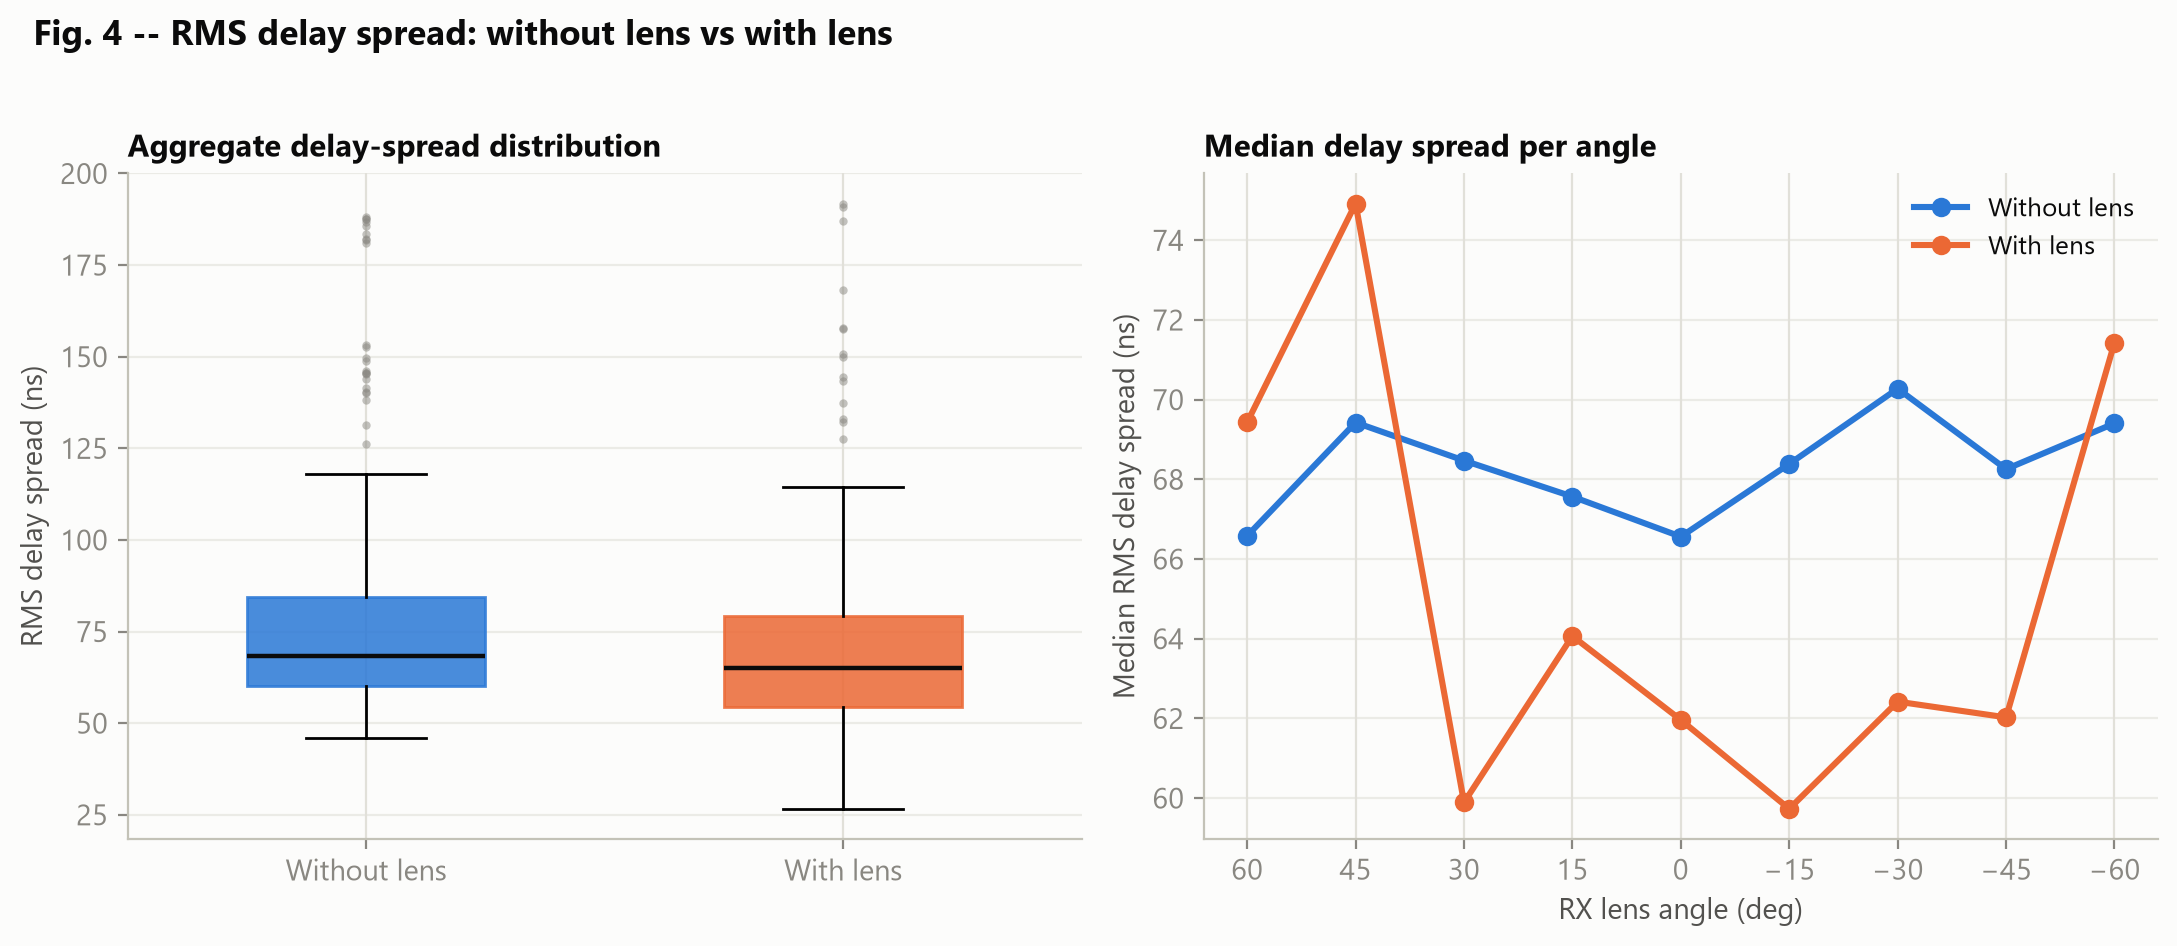
\includegraphics[width=0.85\textwidth]{Images/Eval_20x20_MonteCarlo9x9/asset/figures/fig4_delay_spread.png}
    \caption{RMS delay spread comparison, aggregate and per RX angle, without lens vs.\ with lens.}
    \label{fig:mc9x9-delay-spread}
\end{figure}

The lens reduces median RMS delay spread modestly, from 68.29~ns to 65.01~ns ($-4.8\%$; Table~\ref{tab:mc9x9-delay}, Fig.~\ref{fig:mc9x9-delay-spread}), but the per-angle trend is non-uniform -- delay spread increases at $+45^\circ$ and $-60^\circ$ despite decreasing elsewhere -- indicating that the lens reshapes the power-delay profile in a direction-dependent manner rather than uniformly compressing it.

\begin{table}[htbp]
    \centering
    \caption{RMS delay spread comparison.}
    \label{tab:mc9x9-delay}
    \begin{tabular}{lcc}
        \toprule
        \textbf{Metric} & \textbf{Without lens} & \textbf{With lens} \\
        \midrule
        Median RMS delay spread & 68.29~ns & 65.01~ns \\
        Median paired difference & \multicolumn{2}{c}{$-4.70\,\text{ns}$} \\
        \bottomrule
    \end{tabular}
\end{table}

\subsection{Singular Value, Effective Rank, and Channel Correlation}

\begin{figure}[htbp]
    \centering
    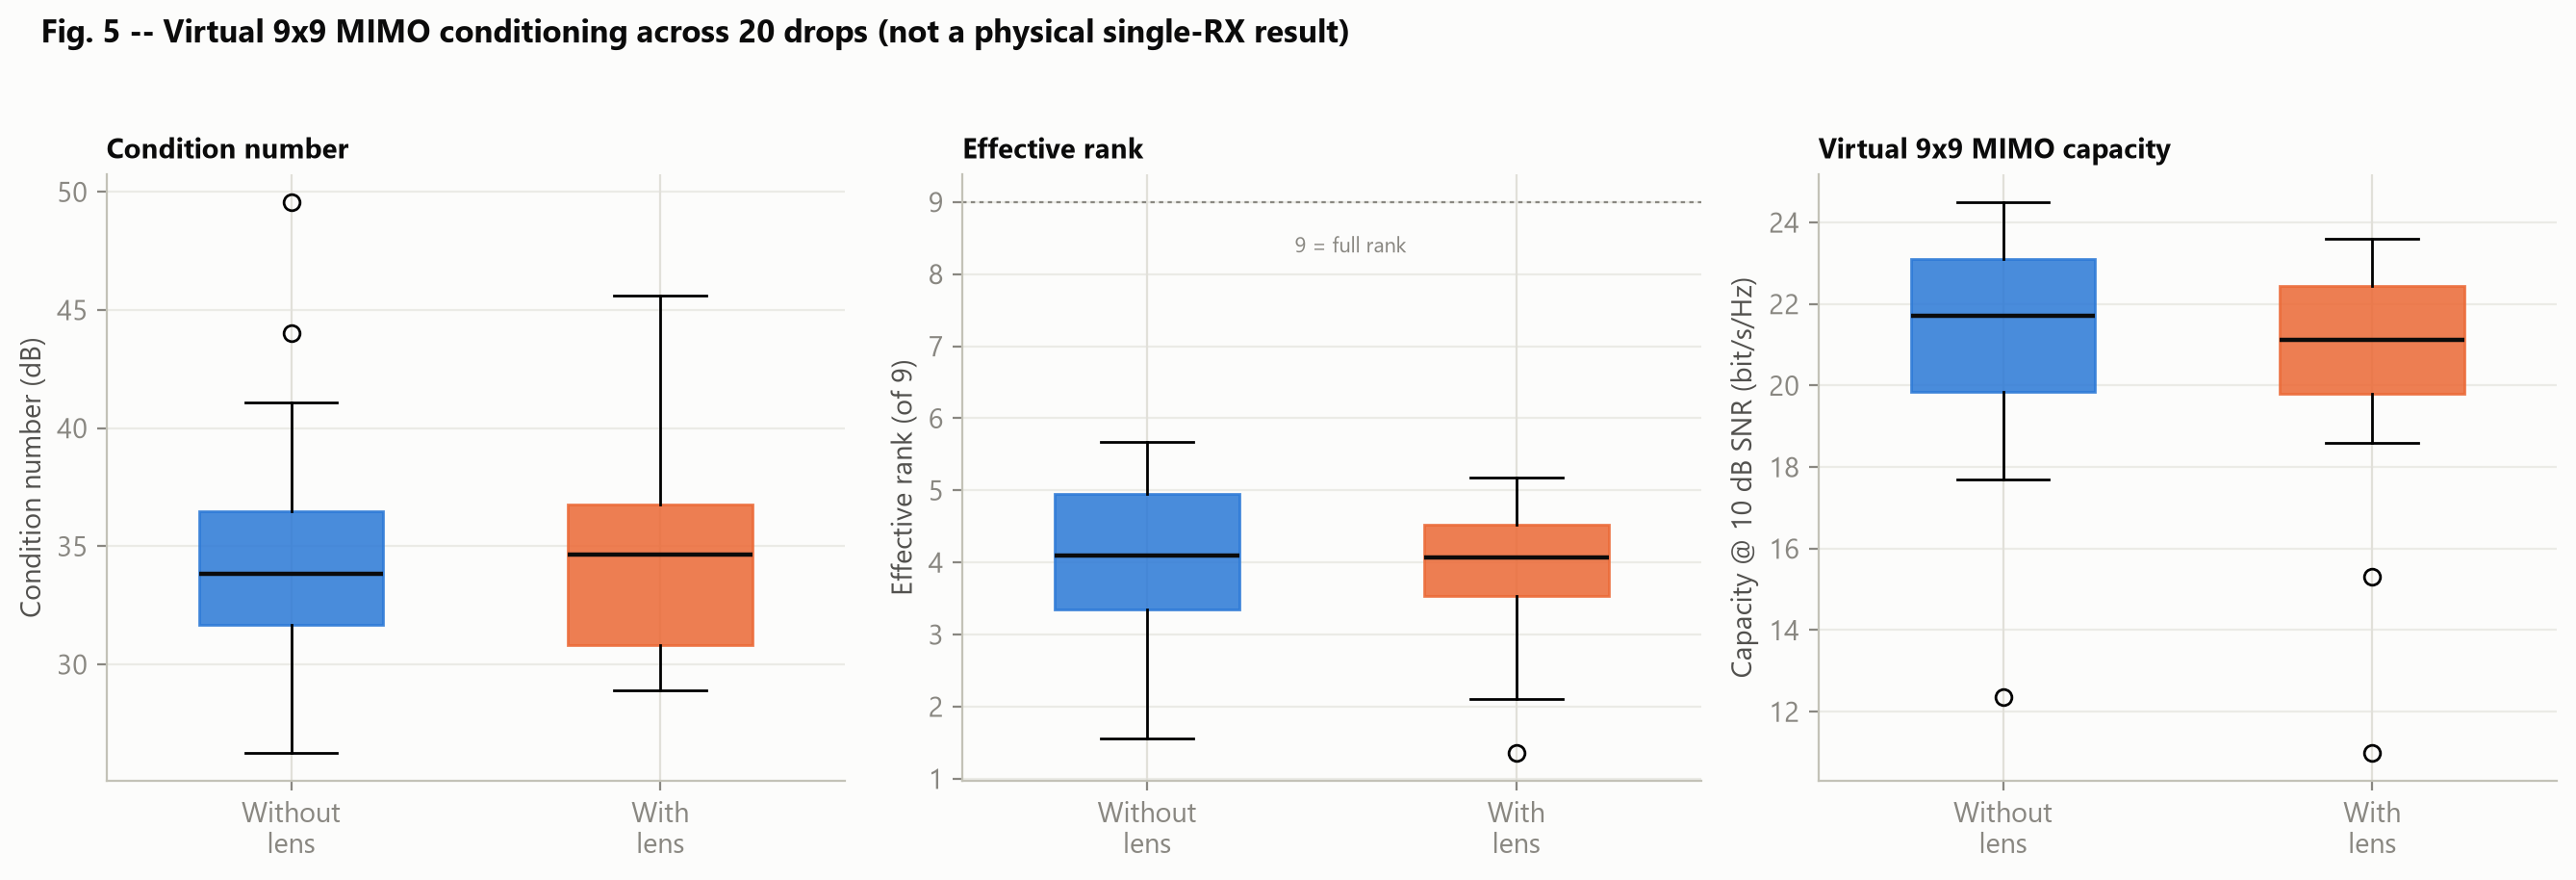
\includegraphics[width=0.85\textwidth]{Images/Eval_20x20_MonteCarlo9x9/asset/figures/fig5_mimo_conditioning.png}
    \caption{Virtual $9\times9$ MIMO channel conditioning: condition number, effective rank, and ergodic capacity at 10~dB SNR, without lens vs.\ with lens.}
    \label{fig:mc9x9-mimo-conditioning}
\end{figure}

The condition number and effective rank of the virtual $9\times9$ channel matrix serve here as diagnostics of channel correlation and spatial-multiplexing potential, since a low effective rank and a high condition number indicate strongly correlated, non-orthogonal eigenmodes. Table~\ref{tab:mc9x9-mimo} and Fig.~\ref{fig:mc9x9-mimo-conditioning} show that the lens does not improve this conditioning: the median condition number increases slightly (49.4 to 54.0, i.e.\ worse), the median effective rank is essentially unchanged (4.09 to 4.07 of 9), and the median virtual MIMO capacity at 10~dB SNR decreases (21.72 to 21.11~bit/s/Hz). This does not contradict the rise in aggregate SISO capacity: a lens can raise received power at specific angles without improving the inter-channel orthogonality that spatial multiplexing depends on.

\begin{table}[htbp]
    \centering
    \caption{Virtual $9\times9$ MIMO channel conditioning.}
    \label{tab:mc9x9-mimo}
    \begin{tabular}{lcc}
        \toprule
        \textbf{Metric} & \textbf{Without lens} & \textbf{With lens} \\
        \midrule
        Median condition number & 49.4 (33.8~dB) & 54.0 (34.6~dB) \\
        Median effective rank & 4.09 of 9 & 4.07 of 9 \\
        Median capacity @ 10~dB SNR & 21.72~bit/s/Hz & 21.11~bit/s/Hz \\
        \bottomrule
    \end{tabular}
\end{table}

\subsection{Discussion of Spatial Multiplexing Capability}

Overall, the antenna lens provides a moderate improvement in typical capacity (median $+5.2\%$) and throughput, together with a small reduction in delay spread, but this benefit is strongly angle-dependent, degrades the 5th-percentile capacity, and yields no improvement in the virtual MIMO channel conditioning that underlies spatial multiplexing. This indicates that, in its present form, the lens functions primarily as an angle-selective power gain mechanism rather than as a means of enhancing channel decorrelation, and that realizing additional multiplexing gain would require deliberate angle and orientation selection together with a larger statistical sample. These conclusions should be interpreted in light of several limitations: a modest number of Monte Carlo drops and path samples relative to recommended practice, an isotropic transmit pattern, transmit power that scales with the number of transmitters, an idealized Shannon capacity bound that excludes modulation, coding, and interference effects, and an angular response that has not yet been independently verified against the physical antenna orientation.

\section{Higher-Order MIMO Systems}

This section examines higher-order lens-assisted MIMO configurations by repeating the Monte Carlo methodology for RX-lens arrays of size $N=3$, $5$, and $9$. All three configurations share an identical room geometry, carrier frequency, bandwidth, transmit power per element, noise figure, and random seed (see the list below). However, increasing $N$ also increases the total transmit power and changes the physical aperture and the set of RX lens angles. The results therefore characterize the combined scaling behavior of the evaluated configurations; they do not isolate array order as the sole causal variable. Because all TX elements radiate simultaneously within a single ray-traced scene, the $N=9$ data point here reproduces the with-lens results already reported in Section~\ref{sec:comparison-antenna-placements}.

\begin{itemize}
    \item \textbf{RX lens-angle scenarios}: $-45^\circ,0^\circ,+45^\circ$ ($N=3$); $-60^\circ$ to $+60^\circ$ in $30^\circ$ steps ($N=5$); $-60^\circ$ to $+60^\circ$ in $15^\circ$ steps ($N=9$)
    \item \textbf{TX array aperture ($Y$)}: $\pm0.45$~m ($N=3$), $\pm0.90$~m ($N=5$), $\pm1.80$~m ($N=9$)
    \item \textbf{Monte Carlo drops}: 20, common to all three array sizes
    \item \textbf{Total Monte Carlo rows} ($20\times N$): 60 ($N=3$), 100 ($N=5$), 180 ($N=9$)
    \item \textbf{Room size, carrier, bandwidth}: $20\,\text{m}\times20\,\text{m}\times3\,\text{m}$; 38~GHz, 400~MHz (401 frequency points)
    \item \textbf{Power per TX / noise figure}: 10~dBm / 7~dB at 290~K
    \item \textbf{Path samples per source}: 100{,}000 (recommended final value: 1{,}000{,}000)
\end{itemize}

\subsection{Compute-Cost Scalability}

Because all TX elements share one radiated pattern and are traced simultaneously within a single scene, the number of \texttt{PathSolver} calls grows linearly with $N$ rather than quadratically as it would if every element were simulated one at a time. Figure~\ref{fig:mc-scalability-compute-cost} contrasts the two schemes for both the fixed-geometry loop and the 20-drop Monte Carlo loop: going from $N=3$ to $N=9$ (a $3\times$ increase in array size), the actual run count also rises $3\times$ (60 to 180 Monte Carlo runs), whereas a naive one-element-per-run scheme would rise $9\times$ (180 to 1620 runs). This linear scaling is what keeps the $N=9$ configuration (180 runs $\times$ 100,000 ray samples) computationally practical.

\begin{figure}[htbp]
    \centering
    
\includegraphics[width=0.85\linewidth]{Analisis_Skalabilitas_MonteCarlo_v3_3x3_5x5_9x9/figures/fig1_compute_cost_scalability.png}
    \caption{Compute-cost scalability: actual vs.\ naive \texttt{PathSolver} run count for the fixed-geometry loop and the 20-drop Monte Carlo loop, for $N=3,5,9$.}
    \label{fig:mc-scalability-compute-cost}
\end{figure}

\subsection{Capacity and Channel-Conditioning Scalability}

Table~\ref{tab:mc-scalability-aggregate} summarizes the aggregate Monte Carlo capacity, throughput, and delay spread, together with the virtual $N\times N$ MIMO conditioning averaged per drop (using the metrics of Equations~\ref{eq:mc9x9-condrank}--\ref{eq:mc9x9-mimocapacity} with $N_t=N$), across the three array sizes.

\begin{table}[htbp]
    \centering
    \caption{Aggregate scalability metrics vs.\ array size $N$ (medians over 20 Monte Carlo drops).}
    \label{tab:mc-scalability-aggregate}
    \small
    \renewcommand{\arraystretch}{1.15}
    \begin{tabularx}{\linewidth}{
        >{\raggedright\arraybackslash}X
        *{3}{>{\centering\arraybackslash}X}
    }
        \toprule
        \textbf{Metric} & \textbf{$N=3$} & \textbf{$N=5$} & \textbf{$N=9$} \\
        \midrule
        Median equivalent-SISO capacity & 5.94~bit/s/Hz & 6.46~bit/s/Hz & 7.67~bit/s/Hz \\
        Median ideal throughput & 2.38~Gbit/s & 2.58~Gbit/s & 3.07~Gbit/s \\
        Median RMS delay spread & 59.13~ns & 63.46~ns & 65.00~ns \\
        Virtual $N\times N$ condition number (per-drop median) & 7.5 (17.5~dB) & 17.1 (24.6~dB) & 54.0 (34.6~dB) \\
        Effective rank / $N$ (per-drop median) & 1.91/3 (64\%) & 2.77/5 (55\%) & 4.07/9 (45\%) \\
        Virtual MIMO capacity @ 10~dB SNR (per-drop median) & 8.03~bit/s/Hz & 12.81~bit/s/Hz & 21.11~bit/s/Hz \\
        \bottomrule
    \end{tabularx}
\end{table}

\begin{figure}[htbp]
    \centering
    
\includegraphics[width=0.9\linewidth]{Analisis_Skalabilitas_MonteCarlo_v3_3x3_5x5_9x9/figures/fig4_montecarlo_aggregate_vs_N.png}
    \caption{Monte Carlo aggregate summary vs.\ array size $N$: (a) median equivalent-SISO capacity with 5th--95th percentile band, (b) median ideal throughput, (c) median RMS delay spread.}
    \label{fig:mc-scalability-aggregate}
\end{figure}

\begin{figure}[htbp]
    \centering
    
\includegraphics[width=0.9\linewidth]{Analisis_Skalabilitas_MonteCarlo_v3_3x3_5x5_9x9/figures/fig5_mimo_per_drop_boxplot_vs_N.png}
    \caption{Per-drop distribution (20 drops) of the virtual $N\times N$ MIMO channel condition number and effective-rank ratio, vs.\ array size $N$.}
    \label{fig:mc-scalability-per-drop}
\end{figure}

Every aggregate metric in Table~\ref{tab:mc-scalability-aggregate} and Figure~\ref{fig:mc-scalability-aggregate} rises monotonically with $N$: more simultaneously active TX elements non-coherently combine at the receiver, raising the received SNR and hence the equivalent-SISO capacity and throughput, while the wider TX aperture at larger $N$ spreads the range of path lengths and raises the RMS delay spread. However, this capacity growth is not free of trade-offs. As Figure~\ref{fig:mc-scalability-per-drop} shows, the virtual $N\times N$ MIMO condition number worsens monotonically with $N$ (17.5~dB $\to$ 24.6~dB $\to$ 34.6~dB), and the effective-rank-to-$N$ ratio decreases monotonically (64\%~$\to$~55\%~$\to$~45\%): although the virtual MIMO capacity at 10~dB SNR keeps rising in absolute terms (8.03~$\to$~12.81~$\to$~21.11~bit/s/Hz), it grows less than proportionally to $N$, since an increasing share of the additional spatial modes are weak or correlated rather than fully independent. This is the classic diminishing-returns pattern of MIMO array scaling: adding lens-steered elements increases the total capacity and link power, but not the proportion of channel dimensions that are genuinely usable for spatial multiplexing.

These conclusions are subject to the same limitations noted in Section~\ref{sec:comparison-antenna-placements} (a modest number of Monte Carlo drops and path samples relative to recommended practice, an idealized Shannon capacity bound, and transmit power that scales with $N$ rather than being held at a fixed total budget), together with one specific to this comparison: the set of RX lens angles tested differs across $N$ (3, 5, and 9 angles, spaced $45^\circ$, $30^\circ$, and $15^\circ$ apart, respectively), so part of the observed variation could stem from the different angular sampling rather than from $N$ alone.


\subsection{Discussion on Higher-Order MIMO Systems}

The higher-order results demonstrate that the adopted simulation strategy remains computationally scalable as the array grows. Increasing the array size from $N=3$ to $N=9$ triples the number of Monte Carlo \texttt{PathSolver} calls, from 60 to 180, rather than increasing it by a factor of nine as in the naive element-by-element approach. Consequently, the ray-tracing cost grows linearly with $N$ because all active TX elements are evaluated simultaneously in each scene. This property makes the analysis of larger arrays practical, although the total post-processing cost and the size of the resulting channel matrices still increase with the number of antenna pairs.

From a communication-performance perspective, a larger array provides a consistent improvement in received-link performance. Between $N=3$ and $N=9$, the median equivalent-SISO capacity increases from 5.94 to 7.67~bit/s/Hz, corresponding to an increase of approximately 29\%, while the median ideal throughput rises from 2.38 to 3.07~Gbit/s. The median virtual-MIMO capacity at 10~dB SNR also increases substantially, from 8.03 to 21.11~bit/s/Hz. These results confirm that adding lens-steered antenna elements introduces additional received power and spatial modes that can be exploited to increase the total achievable rate. The accompanying increase in median RMS delay spread, from 59.13 to 65.00~ns, is comparatively modest but indicates that the larger physical aperture also captures paths with a wider range of propagation delays.

However, the increase in absolute capacity does not imply a proportional improvement in spatial-multiplexing quality. The median condition number deteriorates from 7.5 (17.5~dB) for $N=3$ to 54.0 (34.6~dB) for $N=9$, whereas the normalized effective rank decreases from 64\% to 45\%. Thus, the number of usable spatial modes increases in absolute terms, but more slowly than the number of antenna elements. This behavior suggests that the additional lens directions do not produce fully independent channels; instead, some beams observe overlapping multipath components or similar angular sectors and therefore remain correlated. As the array order increases, power is consequently distributed increasingly unevenly among the singular modes, producing diminishing multiplexing returns.

The observed gains must also be interpreted with care. The transmit power is fixed per element and therefore the total radiated power increases with $N$, so the reported capacity growth combines array-size benefits with an increase in the total power budget. In addition, array aperture and RX angular sampling change together with $N$, preventing the present results from isolating array order as the only causal factor. The use of 20 Monte Carlo drops, 100{,}000 path samples per source, and an ideal Shannon-capacity model further limits the statistical and implementation-level generality of the comparison. A stricter scalability study should hold the total transmit power and physical aperture constant, use a common angular grid, increase the number of drops and path samples, and evaluate practical modulation, coding, and interference assumptions.

In summary, scaling the lens-assisted system to higher-order MIMO is beneficial for total capacity and throughput and is computationally feasible under the simultaneous-source ray-tracing method. Nevertheless, channel conditioning and normalized effective rank worsen as $N$ increases, showing that additional elements alone do not guarantee proportionally more independent spatial channels. The principal design implication is that future higher-order arrays should optimize focal-plane element placement, lens orientation, and beam selection for channel decorrelation, rather than pursuing array size alone. Under the present configuration, higher-order scaling is therefore best characterized as a capacity-enhancing strategy with diminishing spatial-multiplexing efficiency.
